\clearpage
\newpage
\subsection{Local Minima}

Man erreicht das globale Minima nur, wenn man direkt im globalem Minima startet.
Im Endeffekt erreicht man nur in 0.059488\% der Fälle das globale Mimima. In den restlichen Fällen landet man
entweder im lokalem Minima(ebene Fläche im Plot), oder erreicht gar kein Minima(Spitzen im Plot).


\begin{figure}[h!]
  \centering
  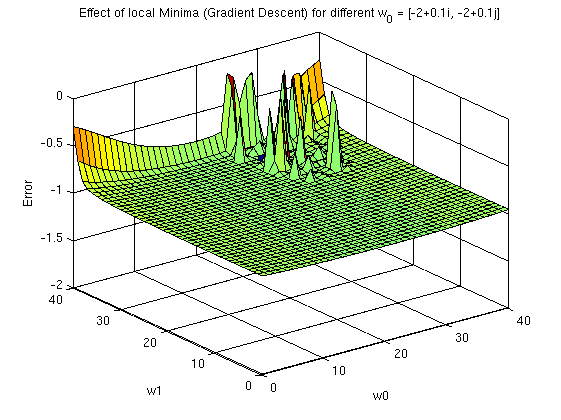
\includegraphics[width=0.8\textwidth]{./figures/214/minf.png}
  \caption{Verlauf von $\vect{w}$}
  \label{fig:minf}
\end{figure}